\section{What is the initiation phase about? Define project goals}
\begin{itemize}
    \item Starts with an idea or need, the person who comes up or identify the need is the project sponsor. 

    \item The responsability of this person are the following:
        \begin{itemize}
            \item Feasibility?
            \item Do we have the resources to complete it?
            \item Will the project deliver the expected benefits?
            \item Appointing a project manager.
        \end{itemize}
\end{itemize}

\subsection{Goal}
\begin{itemize}
    \item Defining a goal, remember the definition of a project, that of a temporary initiative that is agreed, planned, and executed to achieve a specific goal.
    \item  The goal must be worthy of being granted a project.
\end{itemize}

%%%%%%%%%%%%%%%%%%%%%%%%%%%%%%%%%%%%%%%%%%%%%%%%%%%%%%
\section{What is involved in a business case?}  
\begin{itemize}
    \item A business case is a document intended to convince management to invest company resources in this project and not in somebody elses.
    \item It must outline the benefits and the cost (including taxes, inflation, etcetera), the purpose of the project. This is a document that the business leader and project sponsor prepares.
    \item A scope is defined, a scope includes all activities and questions that belong to the project. For example in building a showroom project you might ask wether or not taking pictures of the not yet completed showroom is part of the project, this is a gray area. 
    \item A gray area is questions and situation which arise during the implementation of a project with respect to what is actually part of a project. 
    \item The project team includes production, IT, R\&D, 
    \item A project manager must spot and say in advance and in the initiation phase whether or not something is realistic. If the PM finds a project not feasable the PM must decline to participate in the project.
\end{itemize}

%%%%%%%%%%%%%%%%%%%%%%%%%%%%%%%%%%%%%%%%%%%%%%%%%%%%%%
\section{Who performs the feasability study and what does it involve?}
\begin{itemize}
    \item A business case details all the finances with respect to the project.
    \item A scope outlines what yout project will involve.
    \item A feasability study analyses the goals, scope and the resources to see if they are feasable.
\end{itemize}

\subsection{Feasability study}
\begin{itemize}
    \item The project sponsor and PM should be efficient and analyze this quickly to check generally if the budget is feasable, if the organization posses the needed expertise, do partner companies need to be involved, etcetera.
\end{itemize}

%%%%%%%%%%%%%%%%%%%%%%%%%%%%%%%%%%%%%%%%%%%%%%%%%%%%%%
\section{What goes into risk assesment? What are the expectations?}
\begin{itemize}
    \item Assuming the project is feasable, there are always black swans in the world and bad luck can strike. What are the impacts and risk of this project? This is answered in the risk assesment document.
    \item A risk assesment also checks what an go wrong in order to plan in advance what can we do to mitigate those risks.
    \item This document is also used to outline the expectations, outline who is accountable.
    \item We must spend time with stake holders in order to manage expectations and listen for potential gaps between what is actually being proposed and how to the project is going to look once terminated.
\end{itemize}

%%%%%%%%%%%%%%%%%%%%%%%%%%%%%%%%%%%%%%%%%%%%%%%%%%%%%%
\section{How to create a project charter?}
\begin{itemize}
    \item Assuming the project is still viable despite the risk assesment and feasability.
    \item A project charter is a high level document that is quick and easy to understand. An example:
        \begin{figure}[H]
            \centering
            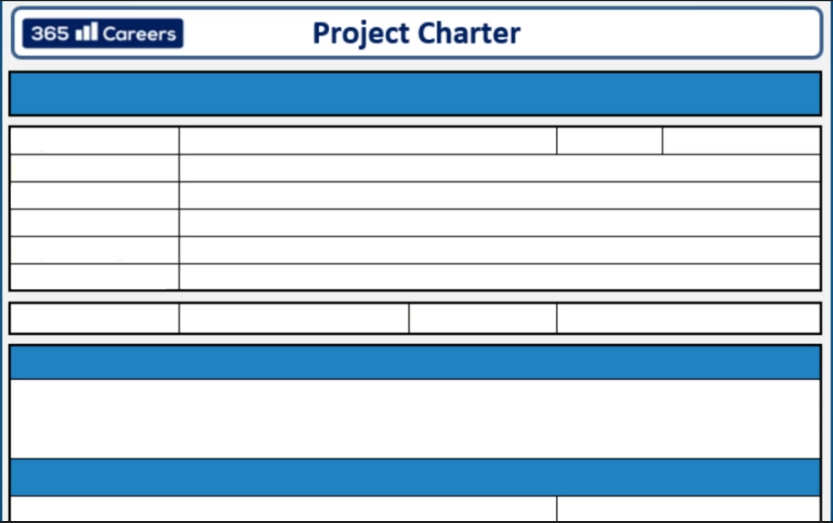
\includegraphics[width=\width\textwidth]{./figs/20221021123941.png}
            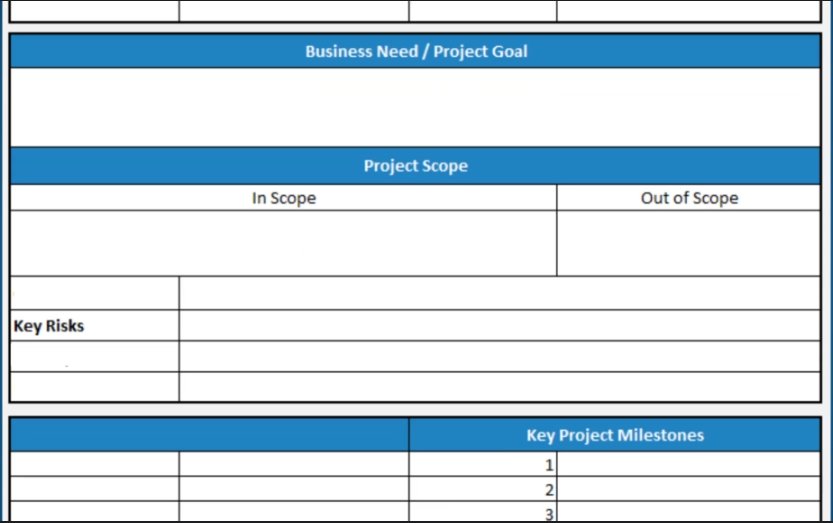
\includegraphics[width=\width\textwidth]{./figs/20221021124023.png}
            %\caption{}
        \end{figure}
    
    \item You can also include the business cases in this document. The important thing is to make this document as easy to read as we can, any one can read it, find what they need and move on. If what they need is more details, the charter will show them where to find the details they need.
\end{itemize}

\subsection{Recap}
\begin{itemize}
    \item Initiation phase is the foundation for the entire project.
    \item The PM can be appointed at any time during the initiation phase so the steps in the initiation phase do not need to be executed in cronological order.
\end{itemize}

%%%%%%%%%%%%%%%%%%%%%%%%%%%%%%%%%%%%%%%%%%%%%%%%%%%%%%
\section{Case study 1}
Outlines the story of an insecure BA that transformed herself into a PM and realized the following: 
\begin{itemize}
    \item No expertise in anything but PM is required to be a PM in a project.
    \item A PM needs to adapt to new environments quickly.
    \item A PM is always learning.
\end{itemize}

%%%%%%%%%%%%%%%%%%%%%%%%%%%%%%%%%%%%%%%%%%%%%%%%%%%%%%
